\chapter{Przedstawienie powiązanych algorytmów}
\label{cha:analizaTeoretycznaProblemu}
Algorytm, którego implementacja jest celem tejże pracy inżynierskiej można podzielić na kilka istotniejszych etapów. Kluczową kwestią jest moment wykrycia twarzy na obrazie, identyfikacja punktów charakterystycznych oraz zastosowanie triangulacji. Właśnie ze względu na  powyższe fakty, w kolejnych podrozdziałach zgłębione zostaną wymienione algorytmy, ich działanie oraz zastosowania. 

\section{Wykrywanie twarzy}
Poprzez pojęcie wykrywania twarzy (ang. face detection) \cite{fDetection} rozumie się opartą o sztuczną inteligencję technologie identyfikującą ludzkie twarze na obrazie cyfrowym. 

Nawiązując do wspomnianych wyżej faktów, owa technika używana jest w wielu rozbieżnych dziedzinach. Nie zawsze spotykamy się z nią świadomie w celu łatwego dostępu do różnego rodzaju sprzętu elektronicznego. Przedstawiana technologia otacza nas wszędzie.

Często wykorzystuje się ją w monitoringu wideo, w celu zapewnienia bezpieczeństwa osobistego jak i narodowego. Co za tym idzie, odpowiednie służby polegają na niej w momencie egzekwowania prawa lub identyfikacji osób w grupie. 

W dziedzinie marketingu zaczęto korzystać z personalizacji reklam dla danego użytkownika. Poprzez integrację kamery internetowej z telewizorem, można gromadzić informacje o osobie, lokalizując ją za pomocą detekcji twarzy. Zbiera się dane dotyczące rasy, płci oraz przedziału wiekowego, aby następnie na tej podstawie dostosować wyświetlane reklamy.

W nowo powstających aparatach fotograficznych wykrywania twarzy używa się podczas automatycznego ustawiania ostrości. Nowoczesne urządzenia przez namierzenie uśmiechu, dobierają odpowiedni moment zrobienia zdjęcia. \cite{fDetection2}

Na przestrzeni lat metody służące wykrywaniu twarzy bardzo się rozwinęły. Na początku używano podstawowych technik przetwarzania obrazów, następnie oparto je na uczeniu maszynowym. Aktualnie ważną rolę w efektywności tejże techniki odgrywają sieci neuronowe, których zastosowanie zdecydowanie przyspiesza działanie programów implementujących ową metodę.

Istnieje wiele różnych propozycji algorytmów służących wykrywaniu twarzy. W celu uporządkowania i pogrupowania metod stosuje się klasyfikację zawierającą cztery podstawowe techniki wykrywania twarzy na obrazie. Dany podział został zaproponowany w 2002 roku przez Ming-Hsuan Yanga (Rys. \ref{fig:detectionMethods}) i obowiązuje do dziś.

\begin{figure}[h]
	\centering
	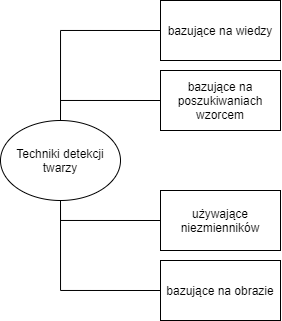
\includegraphics[width=7cm]{techniki-detekcji.png}
	\caption{Techniki detekcji twarzy według Younga.} 
	\label{fig:detectionMethods}
\end{figure}

Charakteryzację każdej z grup \cite{Yang} można przedstawić w następujący sposób:
\begin{itemize}
    \item metody bazujące na wiedzy - wykorzustujące ludzkie obeznanie na temat elementów jakie zawiera przeciętna twarz
    \item techniki używające niezmienników - algorytmy skupiają się na zlokalizowaniu cech strukturalnych twarzy, które są niezmienne ze względu na kąt, oświetlenie, pozycję twarzy
    \item metody bazujące na przeszukiwaniu wzorcem - dzięki wielu zgromadzonym wzorcom odnośnie wyglądu twarzy lub jej konkretnych elementów poszukuje się korelacji między schematem a obrazem wejściowym
    \item metody bazujące na obrazie - model trenowany jest zestawem obrazów, które zawierają różnorodne ludzkie twarze, przedstawiane w zmiennych warunkach
\end{itemize}

Zagadnienie poruszane w tym rozdziale jest bardzo rozległe, a rozwiązania i algorytmy istniejące na rynku bardzo różnorodne. Większość powstałych implementacji łączy najlepsze cechy z kilku metod, przez co nie ma możliwości przypisania ich do konkretnej klasyfikacji. Ze względu na szeroki zakres tej 
tematyki oraz dużą ilość istniejących rozwiązań w dalszej części zostaną opisane dwa najpopularniejsze algorytmy, których implementacje są udostępniane przez biblioteki programistyczne.

\subsection{Schemat działania}
% Algorytmy wykrywania twarzy często postępują w podobny sposób. Większość z nich rozpoczyna swoje działanie od zlokalizowania oczu na obrazie ze względu na ich charakterystyczność. Zdaje się to być najprostszym elementem do wykrycia. \cite{fDetection}

Dla omawianych poniżej algorytmów struktura programu wykrywania twarzy odbywa się dwuetapowo. Początkowym etapem jest wyszkolenie klasyfikatora, którego zadaniem będzie wykrycie twarzy. 

Następnie potrzebne jest działanie detektora skanującego cały obraz w celu lokalizacji istotnych cech takich jak oczy, usta, nos czy brwi. Ich rozpoznanie możliwe jest przez zgromadzone informacje znajdujące się w wytrenowanym wcześniej modelu.

Większość algorytmów uzależnia swoją efektywność od wielkości danych, na których został przeszkolony klasyfikator. Trenowanie na dużych zbiorach danych poprawia zdolność algorytmu w trakcie określenia czy na danym obrazie znajduje się twarz. \cite{fDetection}

\subsection{Klasyfikator kaskadowy z użyciem cech Haara}
Paul Viola i Michael Jones w 2001 roku zaproponowali technikę wykrywania obiektów opartą o działanie klasyfikatora kaskad Haara (ang. Haar Feature-based Cascade Classifier). Pomimo wysokiej konkurencji ze strony sieci neuronowych, algorytm cieszy się ogromną popularnością po dzień dzisiejszy. \cite{haarCascade}Jego zastosowanie okazało się być przełomem w dziedzinie wykrywania twarzy. 

Działanie tej techniki \cite{haar} łączy ze sobą poniższe koncepcje:
\begin{itemize}
    \item poszukiwanie i wybór najdokładniejszych cech Haara
    \item utworzenie zintegrowanych obrazów w celu szybkiego znalezienia danej cechy
    \item użycie metody sprawnego uczenia Adaboost
    \item zastosowanie klasyfikatora kaskadowego
\end{itemize}

Podejście to jest oparte o wytrenowanie klasyfikatora kaskadowego na wielu pozytywnych i negatywnych obrazach w skali szarości. Przez pierwszy rodzaj rozumie się zdjęcia zawierające twarze, natomiast jako próbki negatywne określa się zdjęcia, na których nie znajduje się twarz ludzka. Według zaleceń autorów algorytmu obrazy powinny mieć wymiary $24x24$ pikseli.

Pierwszym krokiem działania opisywanego modelu jest wydobycie ze wszystkich próbek odpowiednich cech Haara. Cechy te dotyczą zmian wartości kontrastu pomiędzy prostokątnymi grupami pikseli. W tym celu wykorzystuje się tak zwane funkcje Haara.

Są to kombinacje prostokątów  o takich samych wymiarach (ciemnych i jasnych), pozwalające na detekcję konkretnych elementów. Funkcje dzielimy na trzy grupy, ze względu na ilość prostokątów (2, 3, 4) tworzących daną cechę. Na Rys. \ref{fig:haarFeatures} przedstawiono funkcje używane w tym algorytmie, wykorzystywane do wykrywania krawędzii na obrazie (1, 2) oraz prostych (3) i skośnych linii (4).

\begin{figure}[h]
	\centering
	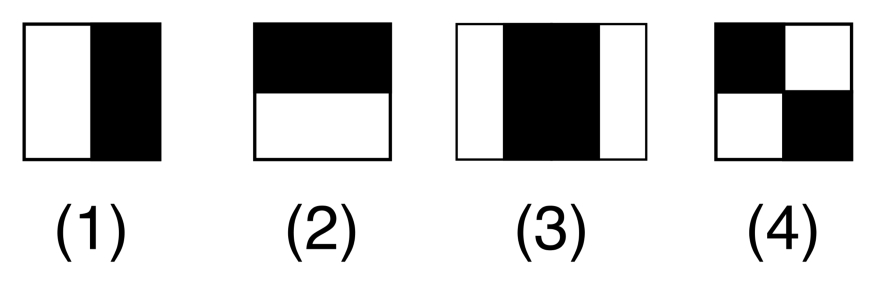
\includegraphics[width=6cm]{haar_features.png}
	\caption{Przykładowe funkcje Haara. \cite{haarCascade}} 
	\label{fig:haarFeatures}
\end{figure}

Każda funkcja Haara przemierza piksel po pikselu dany obraz. Dla każdego regionu (ciemnego jak i jasnego), który obejmuje owa cecha, sumowana jest wartość pikseli znajdujących się w tych obszarach. Następnie obliczana zostaje różnica między tymi sumami. Na podstawie tej różnicy, wyszukuje się lokalizację na obrazie, dla której dana cecha jest najbardziej odpowiednia. 

Przykładowo, na Rys. \ref{fig:haarNose} użyto funkcji złożonej z trzech prostokątów, o rozmiarze mającym na celu wykrycie oczu. Możliwe jest to poprzez fakt, iż obszar oczu jest ciemniejszy niż obszar nosa znajdujacy się pomiędzy nimi. Cechy Haara są pewnego rodzaju wzorcem, dla którego należy znaleźć najlepsze dopasowanie na obrazie.
 
\begin{figure}[h]
	\centering
	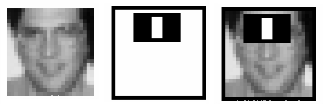
\includegraphics[width=5cm]{haar_nose_feature.png}
	\caption{Zastosowanie funkcji Haara do wykrycia oczu i obszaru nosa.} 
	\label{fig:haarNose}
\end{figure}

Próba dopasowania cech Haara dla każdego piksela zawartego na obrazie, we wszystkich możliwych rozmiarach, wymaga niewyobrażalnej liczby działań. Rozwiązaniem jest stworzenie zintegrowanego obrazu, dzięki czemu złożoność obliczeń staje się dużo korzystniejsza.

Obrazem integralnym nazywamy reprezentację obrazu, w którym dana wartość $(x, y)$ równa jest sumie pikseli znajdujących się powyżej i na lewo od analizowanej lokalizacji (Rys. \ref{fig:integralImage}). Dana reprezentacja pozwala na przyspieszenie działań, jest to skuteczny sposób obliczenia sumy wartości pikseli dla prostokątnego podzbioru rozważanego obrazu.
 
 \begin{figure}[h]
	\centering
	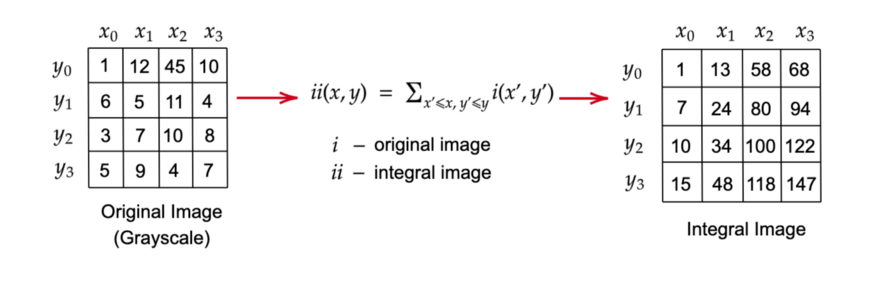
\includegraphics[width=10cm]{integral.png}
	\caption{Konwersja na obraz zintegrowany. \cite{haarCascade}} 
	\label{fig:integralImage}
\end{figure}
 
Kolejnym krokiem jest wybór cech, które są istotne dla konkretnych obszarów. Ten efekt można osiągnąć z pomocą algorytmu Adaboost (ang. Adaptive Boosting). Jest to  algorytm uczenia maszynowego służący do wyboru najlepszych funkcji z całego ich zbioru. Owa technika wzmacniająca, poprzez zastosowanie wszystkich możliwych cech na każdym obrazie treningowym osobno, wybiera te o najniższym błędzie dla danej iteracji. Algorytm trenuje silny klasyfikator na podstawie liniowej kombinacji słabych klasyfikatorów.
 
Po wyborze najlepszych cech spośród wszystkich możliwości pozostaje etap zastosowania klasyfikatora kaskadowego. Z definicji, działa on wielostopniowo. Cechy wybrane jako kluczowe zostają podzielone na grupy, gdzie każda z nich odpowiada jednemu etapowi działania klasyfikatora. Pierwsze etapy zawierają niewiele funkcji, ale wybrane zostają te najbardziej pewne i charakterystyczne. 
 
Funkcje są nakładane na każde okno o zadanych wymiarach wyodrębniane na obrazie. W przypadku negatywnego rezultatu, tzn niedopasowania jednej z cech sprawdzanych w konkretnym etapie, analizowane okno jest od razu odrzucane. Nie rozważa się dla niego funkcji zawartych w dalszych etapach. Jeśli natomiast okno przejdzie pomyślnie wszystkie etapy działania klasyfikatora kaskadowego zostaje zaklasyfikowane jako obszar twarzy (Rys. \ref{fig:cascadeClasificator}).  
 
\begin{figure}[h]
	\centering
	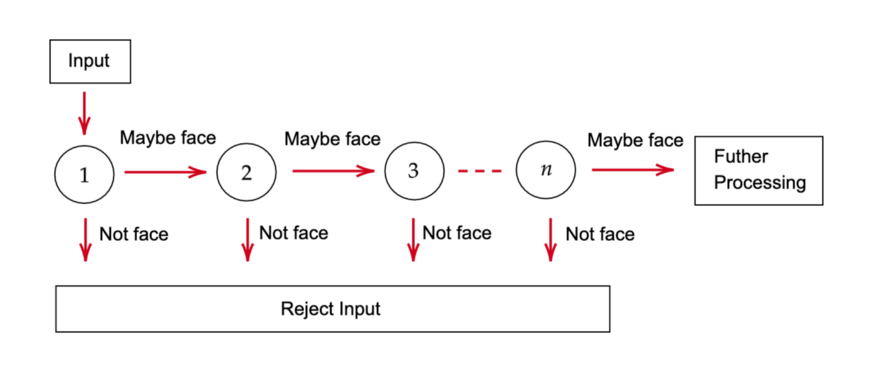
\includegraphics[width=10cm]{haar_train.png}
	\caption{Klasyfikator kaskadowy. \cite{haarCascade}} 
	\label{fig:cascadeClasificator}
\end{figure}

W badaniu przeprowadzonym przez autorów algorytmu wybrano 6000 funkcji, które podzielono na 38 etapów klasyfikacji. Liczba cech w każdym z nich nie jest proporcjonalna, wynosi ona kolejno 1, 10, 25, 25, 50 funkcji dla pięciu pierwszych etapów. W początkowych etapach eliminujemy okna, w których nie ma elementówch charakterystycznych twarzy. Oszczędza to zbędnych obliczeń i analiz.

Opisany w tym rozdziale algorytm jest wykorzystywany nie tylko do wykrywania twarzy na obrazach, ale także innego rodzaju obiektów, takich jak zwierzęta, tablice rejestracyjne czy całe ludzkie sylwetki. 

Cechuje go szybki czas działania oraz dobra poprawność, którą stosunkowo łatwo można zwiększyć. Jest ona powiązana z wielkością zbioru treningowego, na którym został wyszkolony model. Popularność algorytmu, który został opisany w tym rozdziale, zdaje się dalej trwać, pomimo odkrycia wielu konkurencyjnych rozwiązań działających na podobnej zasadzie. 

\subsection{Klasyfikator SVM z użyciem deskryptora HOG}
W 2005 roku pojawiła się kolejna przełomowa propozycja metody wykrywania obiektów, w tym twarzy. Jej autorami są Navneet Dalal i Bill Triggs, którzy wykazali, że do trenowania modelu można skorzystać z deskryptora HOG (ang. Histograms of Oriented Gradients) oraz klasyfikatora SVM (ang. Support Vector Machine). 

Deskryptory wyodrębniają z obrazu przydatne informacje pomijając zbędne dane, pomagają zlokalizować konkretny, interesujący nas obiekt. W przypadku deskryptorów HOG  ekstrakcja cech odbywa się za pomocą histogramu gradientów, używanych jako cechy analizowanych obrazów. Jako gradienty określamy pola wektorowe wskazujące kierunek, w którym można obserwować znaczącą zmianę w intensywności koloru.
%największy wzrost wartości danego pola w poszczególnych punktach.

% Technika ta zlicza występowanie danych gradientów dla określonych fragmentów obrazu. Jej działanie można przedstawić w następujący sposób:
% \begin{enumerate}
%     \item Obraz zostaje podzielony na małe fragmenty
%     \item Dla każdej z komórek oblicza się histogram występowania różnych orientacji krawędzi
%     \item Ostatnim krokiem jest połączenie owych histogramów, przez co otrzymujemy deskryptor HOG dla danego zdjęcia
% \end{enumerate}
% W kolejnych akapitach zostanie zgłębione działanie deskryptora, który odgrywa kluczową rolę w działaniu opisywanego algorytmu.

W celu stworzenia deskryptora HOG dla obrazu należy wykonać kilka istotnych kroków. Pierwszym z nich jest przygotowanie obrazu w odcieniach szarości, dla którego chcemy obliczyć histogram gradientów. Według autorów algorytmu rozmiar zdjęcia powinno się zmniejszyć do $128x64$ pikseli. Takie wymiary zostały wybrane ze względu na początkowe założenie wykrywania obiektów z tymże algorytmem. Miał on służyć do detekcji pieszych. Po sukcesie i dobrych wynikach, skupiono się na detekcji twarzy, w tym przypadku również zdecydowano się na wybór zdjęć o owych wymiarach.

Dla każdego piksela znajdującego się na obrazie należy obliczyć gradient pionowy i poziomy. Najprostszym sposobem jest filtracja obrazu przez poniższe jądra.

\begin{figure}[h]
	\centering
	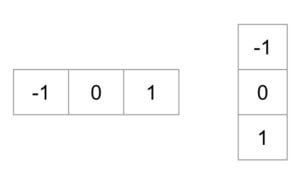
\includegraphics[width=5cm]{hog-kernels.jpg}
	\caption{Jądra służące do filtracji obrazu w celu obliczenia gradientów.} 
	\label{fig:hogKernels}
\end{figure}

Aby znaleźć wielkość i kierunek każdego gradientu w danym bloku używa się określonych wzorów:
\begin{center}
    $g=\sqrt{g_{x}^{2}+g_{y}^{2}}$ ,
    $\theta=\arctan \frac{g_{y}}{g_{x}}$
\end{center}

Kolejnym krokiem jest podział obrazu na jednakowe siatki o wymiarach $8x8$. Każdą komórkę da się przedstawić za pomocą 128 liczb. Pojedynczy fragment składa się z 64 pikseli, z każdym związane są ważne wartości dotyczące jego gradientu - wielkość i kierunek ($8x8x2 = 128$). 

Aby skompresować dane dla każdej siatki, należy stworzyć histogram z podziałem na dziewięć oddzielnych pojemników. Każdy z nich odpowiada kątom z zakresu 0-160 z 20-stopniowym przyrostem.

Przyporządkowując każdy piksel do jednego z pojemników należy kierować się wielkością i kątem gradientu, który go charakteryzuje. Pojemnik jest wybierany ze względu na pierwszy z tych parametrów, natomiast wartość w nim umieszczona zależy od wielkośći. Jeżeli piksel leży w połowie odległości między dwoma pojemnikami, jego wartość dzieli się miedzy oba pola. Omawiana sytuacja dotyczy piksela oznaczonego na czerwono na Rys. \ref{fig:gradientHistogram}. 

Ważną kwestią jest też rozważenie przypadku, gdy analizowany kąt posiada miarę większą niż 160 stopni (maksymalna wartość kąta w pojemniku). W takim przypadku taki piksel dzieli swoją wartość proporcjonalnie z pojemnikiem oznaczonym jako pierwszy.

\begin{figure}[h]
	\centering
	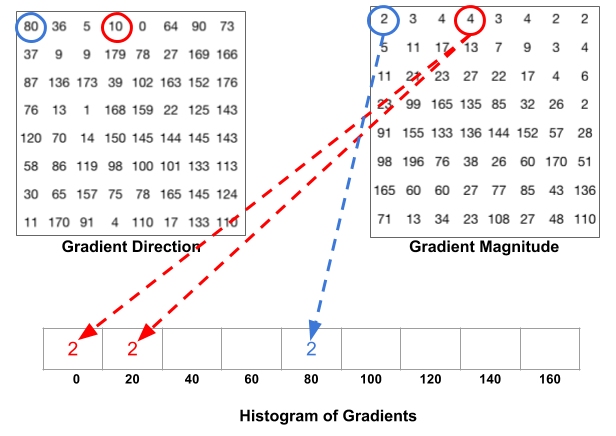
\includegraphics[width=7cm]{gradients-histogram.png}
	\caption{Schemat tworzenia histogramu dla komórki o wymiarach $8x8$.} 
	\label{fig:gradientHistogram}
\end{figure}

Po wykonaniu procesu dla wszystkich pikseli można zobaczyć w jaki sposób rozkładają się wartości w zależności od kąta. Taka reprezentacja zapewnia odporność na szum, którą na początku można zauważyć między gradientami.

Gradienty obrazu są wrażliwe na oświetlenie
Bloki przekształca się w wektory elementów, a następnie stosuje normalizację. Blok o wymiarach $16x16$ posiada 4 histogramy, gdzie każdy da się przedstawić jako wektor $9x1$ co w sumie daje wektor $36x1$. Normalizacja następuje dla pierwszego okna, po czym jest ono przesuwane o 8 pikseli gdzie znormalizowany wektor jest obliczany ponownie. Wszystko powtarza się do momentu przebycia wszystkich pozycji.

Każdy z omawianych bloków reprezentowany jest przez wektor $36x1$ co jest równoznaczne z 36 wyodrębnionymi cechami. Istnieje 105 pozycji takich bloków (7 poziomych, 15 pionowych). Sumarycznie dla naszego zdjęcia otrzymujemy aż 3780 cech.

Powyżej zostało opisane działanie deskryptora HOG na jednym zdjęciu. Jednak celem rozpatrywanego algorytmu, łączącego owe działanie z działaniem klasyfikatorem SVM, jest stworzenie programu wykrywającego twarze.

Klasyfikator SVM pozwala na analizę danych, rozpoznanie wzorców i ich klasyfikację. Do wytrenowania klasyfikatora SVM używa się próbek pozytywnych i negatywnych, tak jak w przypadku przygotowywania klasyfikatora kaskadowego.

Z każdego zdjęcia, za pomocą deskryptora należy wyciągnąć cechy HOG. Na ich podstawie trenuje się klasyfikator SVM. Uczy on się różnych możliwych cech twarzy, które potem próbuje zlokalizować na nowym zdjęciu. Po fazie uczenia, owy klasyfikator pozwala określić do jakiej klasy należą przetwarzane dane. W naszym przypadku rozróżni on fragment zawierający twarz i ten na którym się ona nie znajduje. 


\section{Wykrywanie punktów charakterystycznych}
w sumie no to jesli chodzi o pythona, tooo np te modele od razu tez wykrywaja landmarki jak juz twarz xd too moze ze wzgledu na ich ilosc? jakos porownac czy co, bo iksde w sumie eh joj

\section{Triangulacja Delaunaya}
Poprzez pojęcie triangulacji, w kontekście matematycznym, można rozumieć podział figury geometrycznej na trójkąty, bądź też czworościany (określane jako sympleksy) w taki sposób, aby część wspólna dwóch sąsiadujących trójkątów (czworościanów) była ich wspólną ścianą, wierzchołkiem, bokiem, trójkątem lub zbiorem pustym. \cite{triangulation}

Istnieje wiele różnych rodzajów triangulacji. W przypadku rozważanego w tej pracy algorytmu wykorzystano triangulacje zbioru punktów, do której należy między innymi triangulacja Delaunaya (lub Delone), której nazwa pochodzi od nazwiska autora tejże koncepcji Borysa Delaunaya. 

Triangulacja Delone \cite{tDelone} rozumiana jest jako triangulacja $T$ przestrzeni $R^{n+1}$, którą definiuję się w poniższy sposób.

Jako $T$ określa się podział przestrzeni $R^{n+1}$ na $(n+1)$ sympleksów, z punktami jako wierzchołki, spełniających okreśone warunki:

\begin{enumerate}
    \item każde dwa sympleksy należące do zbioru $T$ posiadają wspólną ściane albo nie są ze sobą połączone w żaden sposób
    \item każdy z ograniczonych zbiorów w przestrzeni $R^{n+1}$ ma część wspólną z ograniczoną liczbą trójkątów ze zbioru $T$
    \item opisując kulę na dowolonym trójkącie ze zbioru $T$ nie natkniemy się na sytuację, gdy wnętrze kuli będzie zawierało wierzchołki z pozostałych sympleksów zawartych w zbiorze $T$
\end{enumerate}

\begin{figure}[h]
	\centering
	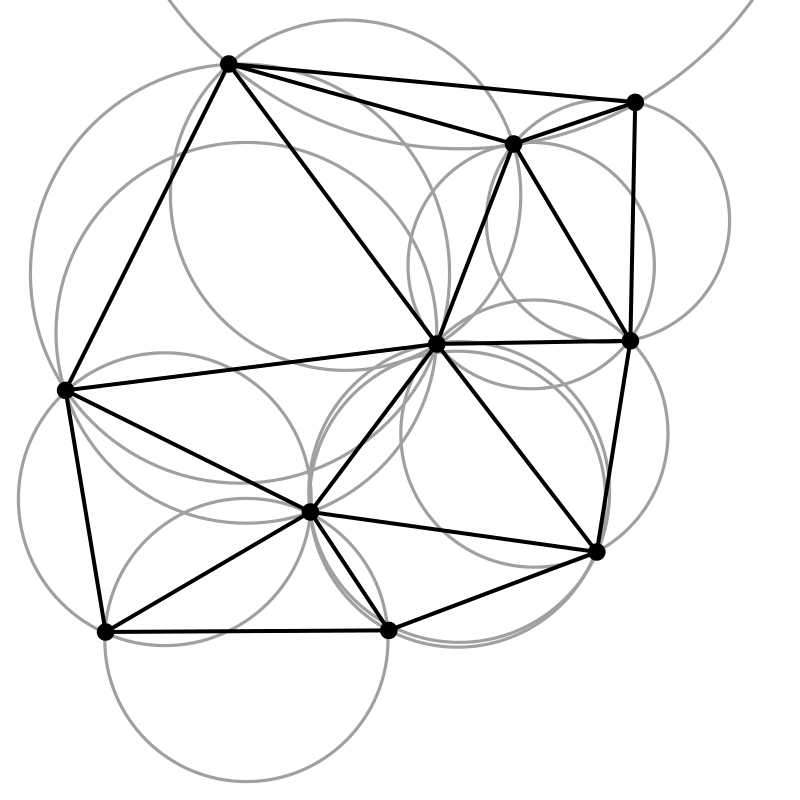
\includegraphics[width=7cm]{triangulation.png}
	\caption{Przykładowa triangulacja Delone dla zbioru punktów. \cite{tDelone}}
	\label{fig:delone}
\end{figure}

Wspominając o triangulacji Delone warto wspomnieć o diagramach Voronoi, które są ściśle powiązane z owym pojęciem. Diagram Voloroi dla zestawu punktów dzieli przestrzeń w taki sposób, że linie podziału znajdują się w równej odległości od punktów sąsiadujących.

Ważną własnością trangulacji Delone jest fakt, iż wraz z diagramem Voronoi tworzy ona graf dualny. Te definicje są powiązane, więc znając trangulację Delone dla zbioru punktów możemy w łatwy sposób obliczyć diagram Voronoi. Dwa trójkąty mające wspólną krawędź w triangulacji umożliwiają odnalezienie krawędzie w diagramie Voronoi. 

Centra okręgów wyznaczonych przez owe trójkąty po połączeniu tworzą daną krawędź. Rys. \ref{fig:voronoi}  przedstawia krawędzie triangulacji (czarne linie) oraz utworzone na podstawie triangulacji komórki Voronoi (czerwone linie).

\begin{figure}[h]
	\centering
	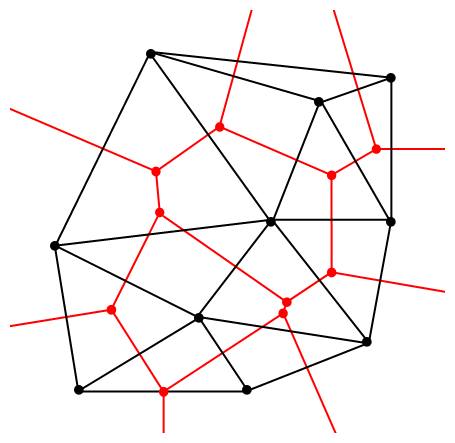
\includegraphics[width=7cm]{voronoi.png}
	\caption{Graf przedstawiający komórki Vornoi oraz krawędzie triangulacji. \cite{tDelone}} 
	\label{fig:voronoi}
\end{figure}

Istotną własnością tej techniki jest fakt, że trójkąty powstałe w wyniku triangulacji nie mają kątów o dużych miarach, co zapewnia przejrzystość wygenerowanych figur. W przypadku zastosowania triangulacji na zbiorze punktów można uniknąć chaosu i nierównomierności.

Triangulacja ma swoje zastosowania w wielu dziedzinach. Wykorzystuje się ją w informatyce, grafice komputerowej czy też geodezji. Technika umożliwia tworzenie skomplikowanych figur, wypełnianie obszarów, wyznaczanie linii przecięcia.

Istnieje wiele różnych algorytmów przeznaczonych do znajdowania trangulacji Delone dla zbioru punktów. Przedstawienie ich w niniejszej pracy dyplomowej nie jest jednak kluczowe. Większość języków programowania dostarcza odpowiednie biblioteki, które posiadają funkcje implementujące takowe algorytmy. 


% Istnieje wiele różnych algorytmów przeznaczonych do znajdowania trangulacji Delone dla zbioru punktów. Nie jest to jednak kluczowe w przypadku niniejszej pracy dymplomowej. W implementacji zostanie użyta odpowiednia biblioteka, która implementuje algorytm triangulacji Delone. 

% W przypadku tworzenia algorytmu animacji awatara istotne jest, aby trójkąty tworzone ze zbioru punktów charakterystycznych były zbudowane w odpowiedni sposób. Trójkąty powstałe w wyniku triangulacji nie będą mieć dużych kątów, co zapewni przejrzystość powstałych figur. W przypadku podziału twarzy na takowe figury unikniemy chaosu, nierównomierności. Właśnie dlatego zdecydowałam się na wybór tejże techniki.


